\begin{frame}
\frametitle{Buddy аллокатор}
\begin{itemize}
    \item<1->Buddy аллокатор предназначен для аллокации больших участков памяти
    \begin{itemize}
        \item<2->buddy аллокатор аллоцирует память блоками;
        \item<3->блок - $2^i$ последовательных страниц;
        \item<4->например, 1 страница, 2 страницы, 4 страницы и т. д.;
	\item<4->но не 3 страницы или 5 страниц.
    \end{itemize}
\end{itemize}
\end{frame}

\begin{frame}
\frametitle{Дескрипторы страниц}
\begin{itemize}
    \item<1->Buddy аллокатор не будет работать с памятью напрямую
    \begin{itemize}
        \item<2->вместо страниц памяти будем использовать в алгоритме
        дескрипторы;
        \item<3->просто массив дескрипторов - по адресу страницы легко получить
        дескриптор и наоборот.
    \end{itemize}
\end{itemize}
\end{frame}

\begin{frame}
\frametitle{Дескрипторы страниц}
\begin{itemize}
    \item<1->Что будет храниться в дескрипторах?
    \begin{itemize}
        \item<2->указатели, чтобы связать дескрипторы в двусвязный список;
        \item<3->признак свободности/занятости;
        \item<4->уровень (указание на размер блока).
    \end{itemize}
\end{itemize}
\end{frame}

\begin{frame}
\frametitle{Списки свободных блоков}
\begin{itemize}
    \item<1->Пусть у нас изначально есть $2^N$ последовательных свободных
    страниц:
    \begin{itemize}
        \item<1->заведем $N + 1$ изначально пустой двусвязный список;
        \item<1->$i$-ый список будет хранить свободные блоки размером $2^i$
        страниц.
    \end{itemize}
\end{itemize}
\end{frame}

\begin{frame}
\frametitle{Начальное состояние}
\begin{itemize}
    \item<1->Возьмем дескриптор $0$-ой страницы
    \begin{itemize}
        \item<2->отметим дескриптор как свободный;
        \item<3->зададим в дескрипторе уровень $N-1$;
        \item<4->добавим дескриптор в список $N-1$.
    \end{itemize}
\end{itemize}
\end{frame}

\begin{frame}
\frametitle{Инициализация}
\includegraphics[height=.43\textheight]{bud0}
\end{frame}

\begin{frame}
\frametitle{Аллокация}
\begin{itemize}
    \item<1->Мы хотим аллоцировать $2^i$ страниц
    \begin{itemize}
        \item<2->найдем непустой список с блоками $\ge 2^i$;
        \item<3->берем один из блоков и делим его пополам, пока не останется
        $2^i$.
    \end{itemize}
\end{itemize}
\end{frame}

\begin{frame}
\frametitle{Аллокация}
\includegraphics[height=.43\textheight]{bud0}
\end{frame}

\begin{frame}
\frametitle{Аллокация}
\includegraphics[height=.43\textheight]{bud1}
\end{frame}

\begin{frame}
\frametitle{Аллокация}
\includegraphics[height=.43\textheight]{bud2}
\end{frame}

\begin{frame}
\frametitle{Аллокация}
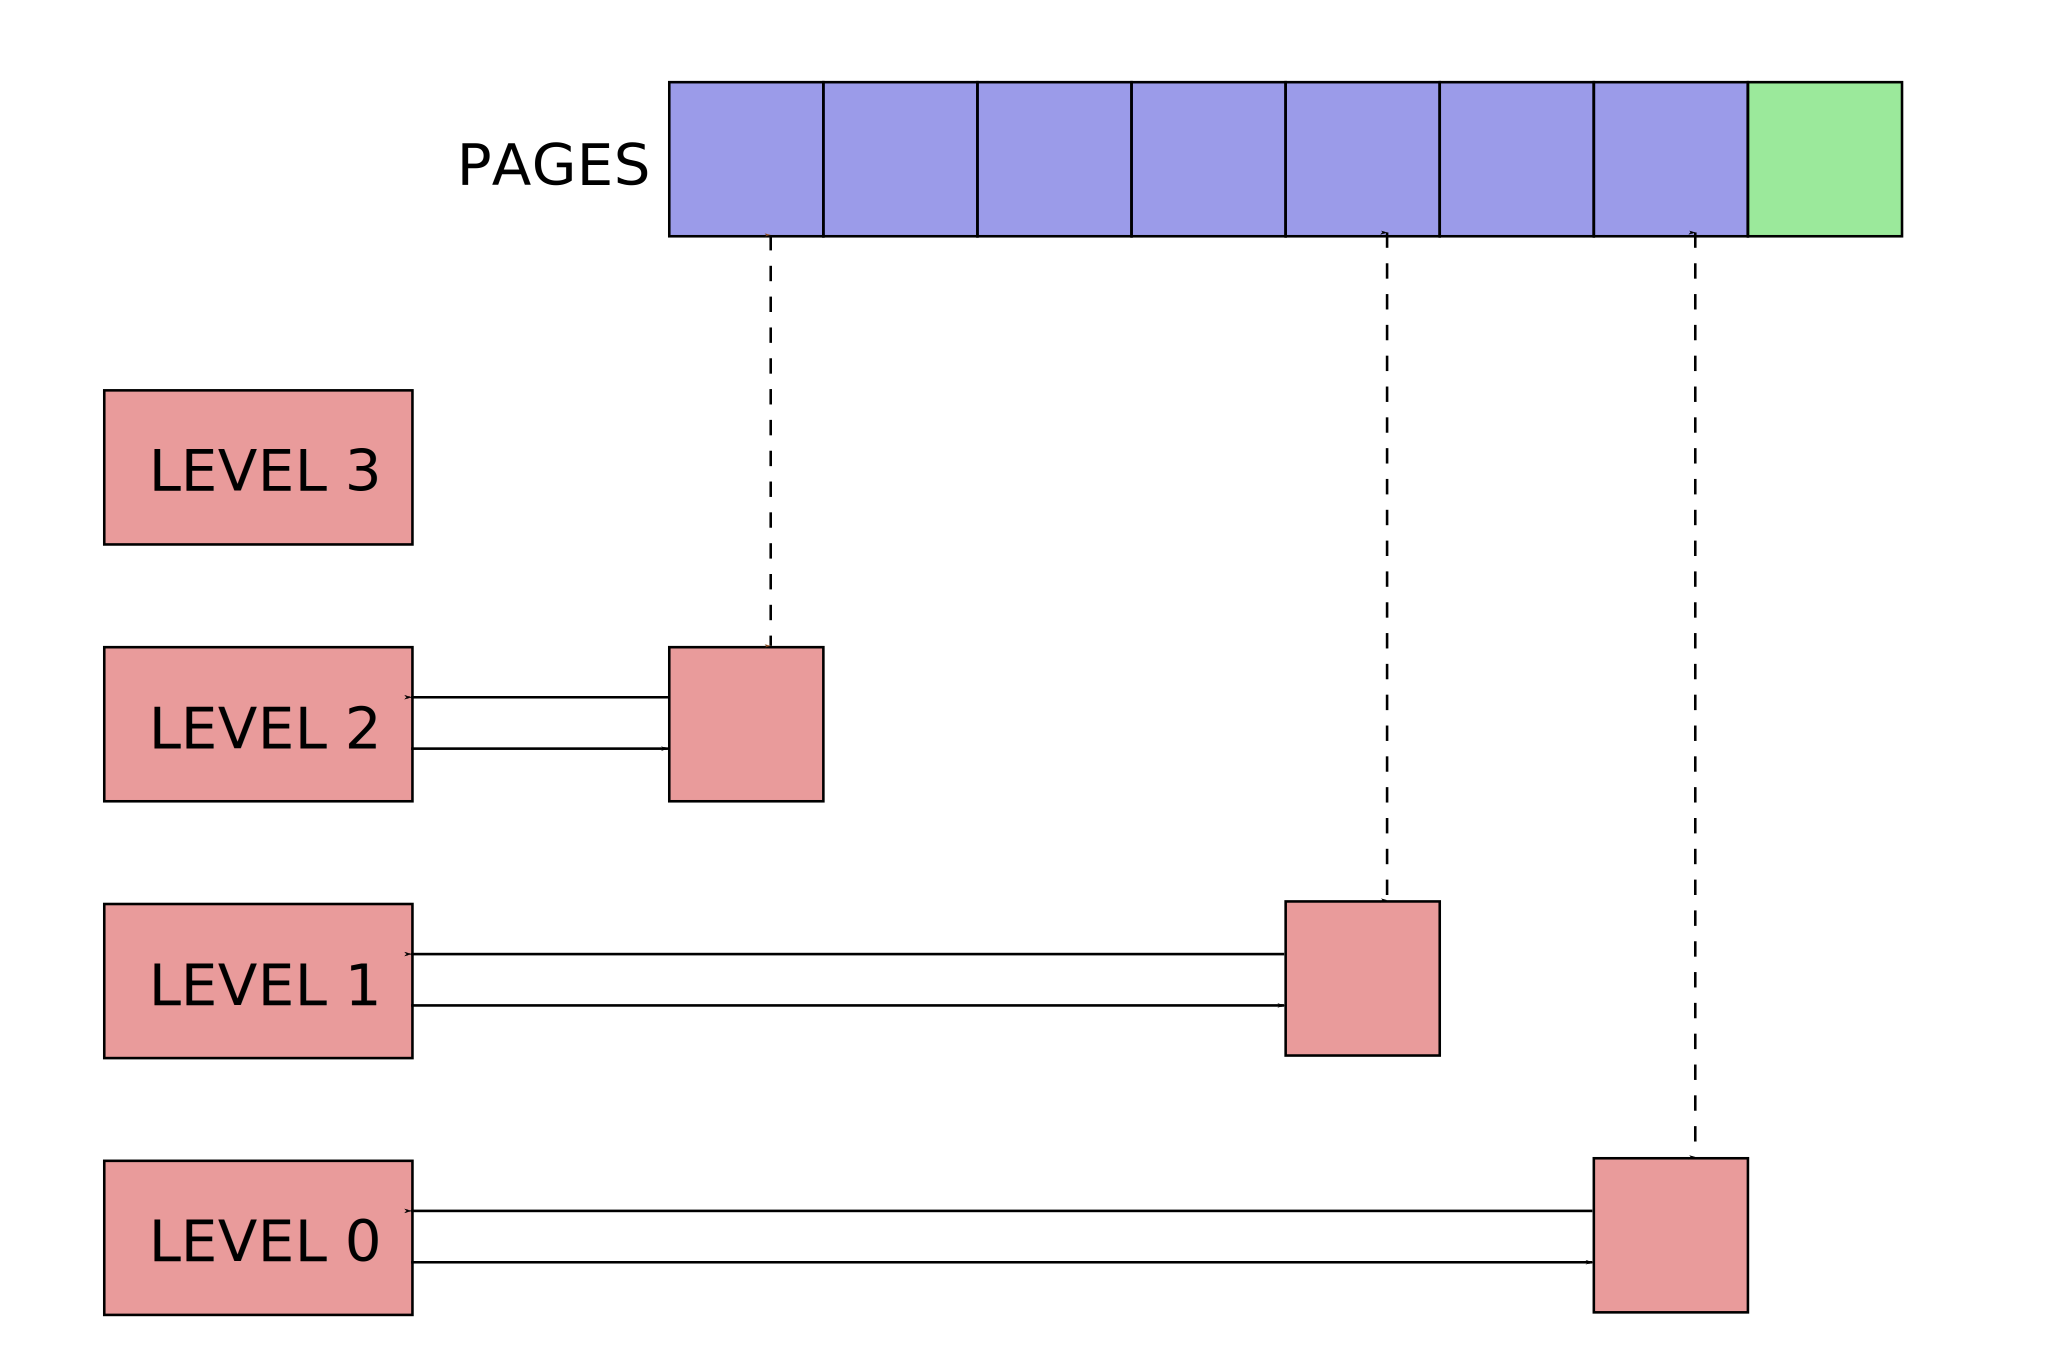
\includegraphics[height=.43\textheight]{bud3}
\end{frame}

\begin{frame}
\frametitle{Освобождение}
\begin{itemize}
    \item<1->Теперь мы хотим освободить блок размера $2^i$
    \begin{itemize}
        \item<2->мы могли бы просто добавить дескриптор в список $i$, но это
        приведет к фрагментации;
        \item<3->мы должны попытаться объединить смежные блоки.
    \end{itemize}
\end{itemize}
\end{frame}

\begin{frame}
\frametitle{Buddies}
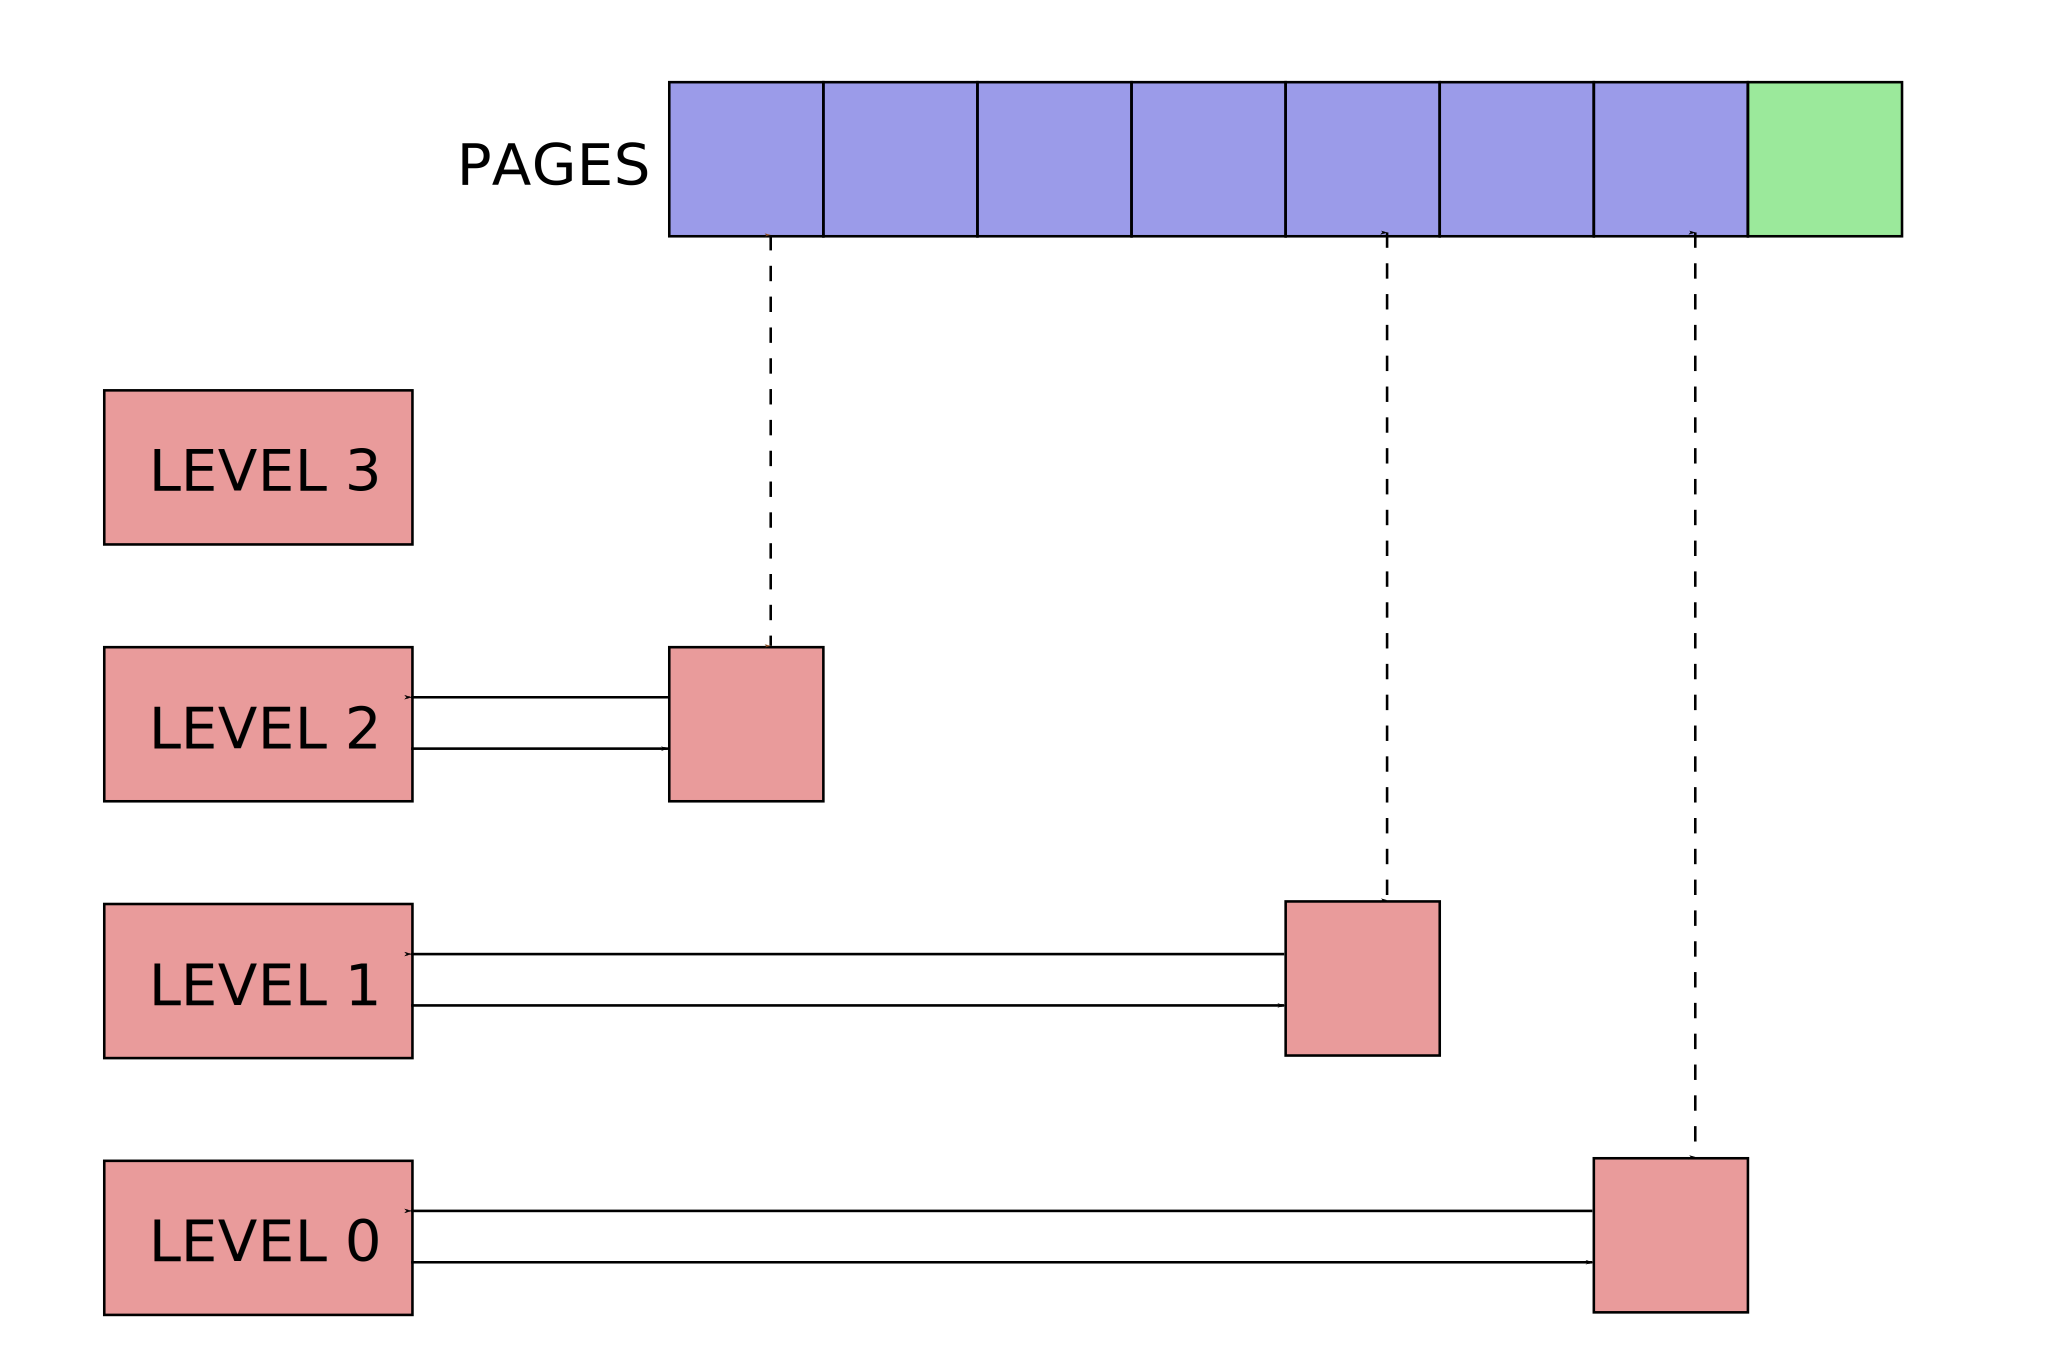
\includegraphics[height=.43\textheight]{bud3}
\end{frame}

\begin{frame}
\frametitle{Buddies}
\begin{itemize}
    \item<1->Как найти парный блок?
    \begin{itemize}
        \item<1->если мы осовобождаем блок размера $2^i$ с номером $j$;
        \item<2->парный блок имеет номер $j \oplus 2^i$;
	\item<2->$\oplus$ - исключющее побитовое ИЛИ.
    \end{itemize}
\end{itemize}
\end{frame}

\begin{frame}
\frametitle{Освобождение}
\begin{itemize}
    \item<1->Когда можно объединять парные блоки?
    \begin{itemize}
        \item<2->если оба блока свободны;
        \item<3->если оба блока имеют один размер (уровень в дескрипторе).
    \end{itemize}
\end{itemize}
\end{frame}

\begin{frame}
\frametitle{Освбождение}
\includegraphics[height=.43\textheight]{bud4}
\end{frame}

\begin{frame}
\frametitle{Buddies}
\includegraphics[height=.43\textheight]{bud5}
\end{frame}
